\documentclass{../../text-style}

\texttitle{Лекция 5: Управление проектом}

\begin{document}

\maketitle
\thispagestyle{empty}

\attribution{По материалам Тимофея Александровича Брыксина, бывшего доцента кафедры системного программирования СПбГУ}

\section{Отслеживание прогресса}

Для того, чтобы уметь адекватно управлять ходом проекта, менеджер должен понимать, в каком состоянии сейчас проект, как в плане сроков разработки, так и в плане затрат. В этом деле первое, что важно понимать~--- ничто никогда не идёт по плану. Но как отклонение по срокам такой-то задачи отразится на общем ходе проекта, его сроках и стоимости, и к чему это приведёт в плане бизнес-задач проекта (да даже есть это отклонение или нет)~--- вопрос, на который для достаточно больших проектов невозможно так сразу ответить. Требуется наладить механизм отслеживания прогресса и, возможно, считать численные метрики, которые позволят понять, как идут делаю

\subsection{Механизмы отслеживания}

\subsubsection{Отслеживание задач}

Наверное, самый важный инструмент отслеживания~--- это адекватная иерархическая структура работ (Work Breakdown Structure, WBS), с оценкой по каждой задаче. Без вменяемых оценок нельзя предсказать с достаточной точностью даже планируемую дату завершения проекта, не то что насколько мы укладываемся в сроки.

Следует стараться делать задачи небольшими, иначе отслеживать их прогресс будет очень сложно (стоит руководствоваться правилом 8-80, упоминавшемся в предыдущей лекции~--- задача не должна иметь оценку меньше 8 часов и более 80 часов, но с поправкой на размер проекта). Кроме того, у каждой задачи должен быть очевидный критерий завершенности, чтобы однозначно определять, когда задачу можно закрыть.

Важно также иметь возможность оценить прогресс по каждой задаче. Лучше всего это делать с помощью трекера задач (Jira, Yandex Tracker, GitHub Projects и т.п.), и ввести в команде правило, что \emph{любая} задача должна \emph{вовремя} отмечаться как взятая в работу или сделанная. И строго это контролировать. Плюс к тому, при тактическом планировании (например, при планировании спринта в Scrum) не терять информации, откуда появилась та или иная задача (например, задача из WBS может становиться эпиком в Scrum и декомпозироваться на конкретные задачи длительностью 2-3 часа в бэклоге спринта, либо можно просто ссылаться на исходную задачу во \emph{вспомогательных}, выявленных при планировании спринта).

Также может быть полезно отслеживать статус задач на ежедневных митингах (если ваша организация такое не практикует, то в еженедельных отчётах). В этом случае можно собрать больше информации о статусе задачи, чем просто \enquote{не брались/делаем/сделали}, однако стоит избегать соблазна просить у разработчиков точный процент, на который задача сделана. Разумнее всего следовать правилу \enquote{0-50-100}, которое говорит, что у задачи есть только три варианта процентов завершения~--- 0\% (не приступали или только начали), 50\% (делаем, вроде сделали больше половины), 100\% (сделали). Вам как менеджерам приятно было бы иметь более точную информацию о прогрессе, но вы как разработчики должны понимать, что любая задача 80\%  времени сделана на 80\%, так что более точная информация бесполезна. Точная оценка статуса проекта берётся из того факта, что задач в WBS много.

\subsubsection{Отслеживание статуса по людям}

Из таск-трекера также можно извлечь много информации персонально по поводу каждого конкретного разработчика. Сколько задач конкретный человек сделал, сколько переоткрыл, сколько сейчас на нём висит, переработка/недоработка, и т.д. Например, если у программиста недоработки и большое количество переоткрытых задач, то, скорее всего, он работает неэффективно и нужно привлечь его внимание к этому вопросу.

Также хорошей практикой являются еженедельные отчеты. Обычно они оформляются в виде таблички, в которой указаны задачи, которыми человек занимался, и количество часов на каждую. С таким видом статистики следует быть осторожным, т.к. на практике менеджер часто хочет увидеть в этой табличке строго 40 рабочих часов за неделю. Не стоит так делать, поскольку если заставить людей писать \enquote{40}, то они и будут писать \enquote{40}, а такая статистика вряд ли будет соответствовать действительности, т.к. люди будут подгонять время под это количество часов. Как показывает практика, в реальной жизни получается не 8 часов в день, а немного меньше. Поэтому, если проект идет по графику и результат получается хорошим, то 40 часов в неделю может и не быть (и это не страшно). Фраза \enquote{должно быть 40} всегда всё портит. Если же этого избегать, то программисты не будут пытаться натянуть свой график на эти мифические 40 часов. Соответственно, оценки будут честные.

Следует также сказать, что написание отчетов дисциплинирует программистов (несмотря на то, что они будут этому активно сопротивляться), а для менеджера такие отчеты очень важны для сбора и анализа данных. Если есть возможность генерации подобных отчетов из таск-трекера вместо ручного заполнения~--- это большой плюс.

Если в проекте Scrum (или любая другая Agile-методология) и самоорганизующаяся команда, то в еженедельных отчётах, как правило, нет нужды. Может учитываться фактически отработанное время (то, что часто называют \enquote{табелем}), но это сугубо формальная штука, на основании которой начисляют зарплату~--- это не про \enquote{Твой рабочий день начинается в 9:00, а не в 9:03!}, а про больничные и отгулы. Если не выплатить зарплату за неотработанные три минуты времени, больше потратите на суды и штрафы от разных органов защиты прав работника, трудовой кодекс к работодателю довольно суров.

\subsubsection{Отслеживание дефектов}

Аналогично людям и задачам, только по известным ошибкам и прочим дефектам: общее количество дефектов, относящихся к сотруднику; количество незакрытых дефектов, относящихся к сотруднику; среднее время исправления дефекта; процент переоткрытых дефектов; распределение дефектов по модулям/компонентам, приоритетам, статусам; количество дефектов для каждой задачи и т.п.

Важно правильно интерпретировать эту метрику. Идея, что проект имеет N открытых дефектов в трекере, его пора закрывать, может быть весьма неудачной, потому что дефекты в трекере~--- это дефекты, которые \emph{нашли}, а значит, продукт кому-то был нужен (ну или у вас реально хороший тестировщик завёлся). Мало дефектов может свидетельствовать как о высоком качестве кода, так и о низком качестве тестирования при отсутствии пользователей.

\subsubsection{Отслеживание коммитов}

При оценке производительности программиста по коммитам важно учитывать многие факторы. Во-первых, важно не количество коммитов, а их содержательная часть. Просто считать коммиты или количество измененных строчек~--- не лучший подход, поскольку изменения бывают разные (например, можно просто заменить все пробелы в проекте на символы табуляции. Количество строчек будет огромным, а их практическая ценность нулевой). У всех разный стиль разработки, но всё же обычно есть общепринятая культура в команде, так что интересно смотреть на время коммитов, их регулярность.

\subsubsection{Графики}

При анализе каких-то численных показателей следует смотреть на общую динамику изменений. Не стоит смотреть на цифры в отдельности, т.к. это не слишком наглядно.

Например, рассмотрим два графика: по планируемой/выполняемой работе и по затратам:

\begin{center}
    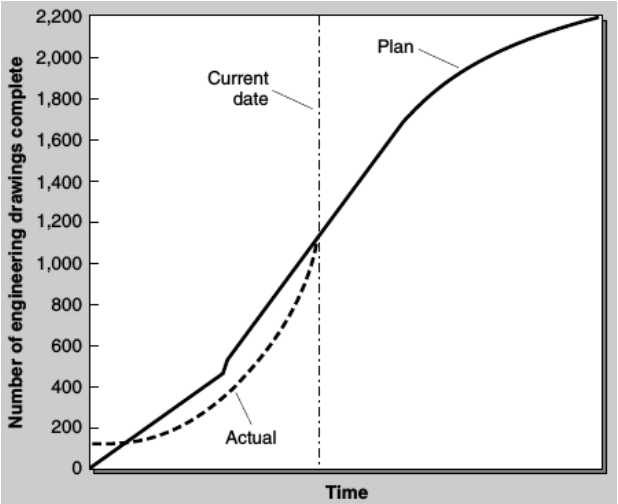
\includegraphics[width=0.5\textwidth]{plannedWorkGraph.png}
\end{center}

\begin{center}
    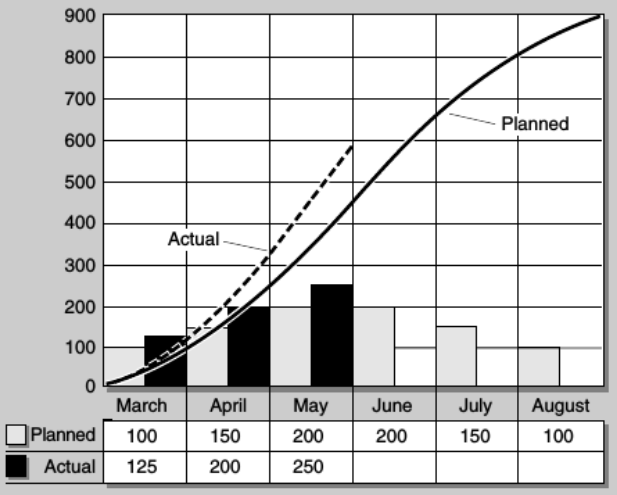
\includegraphics[width=0.5\textwidth]{costGraph.png}
\end{center}

Оба графика показывают изменение показателей во времени, но у них есть свои недостатки. Первый график плох тем, что в нем не учитывается сложность задач. Он показывает лишь то, что команда отстает, а в какой-то момент догоняет исходный план. Но это не показывает, какие задачи были сделаны~--- возможно, самые простые, а может быть и самые сложные.

Второй график~--- график расходов~--- показывает, что команда тратит больше, чем нужно, но, возможно, было выполнено гораздо больше запланированной работы.

Для полноты картины нужно смотреть на происходящее в проекте со всех сторон, иначе особого смысла нет. Без контекста подобную информацию можно с лёгкостью интерпретировать неверно.

Как обычно, ценным инструментом визуализации следования графику работ служат диаграммы Гантта. На \enquote{полосках}, визуализирующих задачу, можно откладывать прогресс, заштриховывая процент \enquote{полоски}, на который задача сделана. Если все задачи слева от текущей даты \enquote{закрашены}, мы укладываемся в график. Но помним, что точно померить степень выполненности задачи невозможно, поэтому такая визуализация для текущих задач не очень информативна (зато вполне хорошо работает для уже законченных или ещё не начатых).

\subsection{Метрики}

Всё, описанное выше, относится к сбору данных, местами их визуализации и качественной оценке, но для больших проектов это мало что даёт в силу большой сложности взаимосвязей между самими задачами, и задачами и разными другими показателями, главными из которых являются финансовые потоки. Хочется иметь набор численных показателей, которые можно объективно измерять, которые достаточно информативны, которые можно предсказывать или выбирать в качестве целевых. Собственно, в теории управления проектами таких метрик придумано довольно много, они применяются далеко не только в IT и в целом считается что хорошо работают.

Метрики собирают для того, чтобы прежде всего принимать на их основе решения. То есть считать какой-то численный показатель только потому, что почему нет~--- плохая идея. Самые важные показатели, которые влияют на управление проектом~--- это насколько мы укладываемся в календарный график и насколько мы вписываемся в бюджет проекта. Кроме этого метрики помогают понять использование ресурсов (трудовых и материальных), удовлетворённость пользователей и т.п.

Любые измерения~--- это дополнительная работа для менеджера проекта, причём зачастую весьма немаленькая, поэтому метрики надо осознанно выбирать так, чтобы они были полезны (то есть, опять-таки, на их основе можно было принимать содержательные решения). Хорошие метрики должны удовлетворять уже знакомы нам критериям SMART, которые мы применяли для оценки \enquote{качества} задач в WBS:

\begin{itemize}
    \item Specific~--- должно быть понятно, что конкретно мы измеряем, и как мы это делаем;
    \item Meaningful (в отличие от аналогичного пункта критерия у задач, там было Measureable)~--- метрика должна характеризовать бизнес-цели, достижение требований и т.п., то есть быть осмысленной для проекта;
    \item Achievable~--- если для метрики задан целевой показатель, он должен быть достижимым;
    \item Relevant~--- метрика должна быть такой, чтобы на её основании можно было принимать содержательные решения (тут некое перекрытие с \enquote{Meaningful}, но SART звучало бы хуже);
    \item Timely (в отличие от аналогичного критерия для задачи, там оно было Time bound)~--- метрика должна характеризовать текущее или будущее состояние дел, считаться оперативно.
\end{itemize}

Есть некоторые типовые метрики, которые перечислены в Project Management Body Of Knowledge (PMBOK), условно разделяемые на следующие категории:

\begin{itemize}
    \item Технические метрики~--- если приложение уже эксплуатируется, их можно собирать по продуктовому окружению. Например, количество пользователей, количество \emph{конверсий} (то есть пользователей, которые не просто воспользовались вашим приложением, а сделали в нём что-то вам полезное, например, заказали товар в интернет-магазине), число ошибок в секунду, использование процессора и оперативной памяти и т.п. Таких метрик десятки, большая часть из них специфична для приложения, поэтому мы тут про них говорить не будем. Есть общепринятые технические показатели для веб-приложений, например, RED (Requests-Errors-Duration, запросов в секунду/ошибок в секунду/среднее время обработки одного запроса), но про них стоит говорить на курсе по архитектуре.
    \item Метрики хода разработки~--- тоже на самом деле много разных метрик, которые характеризуют, как команда работает. Они уже более интересны менеджеру, так что про них ниже подробнее.
    \item Метрики использования ресурсов~--- характеризуют использование ресурсов проектом (трудовых или материальных), например, загруженность разработчиков. Важные, но простые и понятные (значимых на самом деле всего две~--- загруженность ресурсов и стоимость ресурсов относительно заложенной в бюджете), так что дальше обсуждать их не будем.
    \item Метрики стоимости и графика~--- разные показатели, описывающие состояние проекта относительно изначально планировавшегося графика работ и бюджета. Пожалуй, ключевые для стратегического управления, хоть и сложно считаются, и там больше десятка странных аббревиатур, в которых легко запутаться.
    \item Бизнес-метрики~--- метрики, характеризующие самые высокоуровневые бизнес-цели проекта, обычно показывают, стоит ли вообще за проект браться или стоит ли его продолжать.
    \item Удовлетворённость ключевых участников~--- субъективные метрики, оценивающие то, насколько все всем довольны. Прежде всего пользователи, но также важна и команда.
    \item Прогнозные метрики~--- метрики, позволяющие предсказать результаты проекта в финансовом и/или временном плане.
\end{itemize}

\subsubsection{Метрики хода разработки}

Метрики, характеризующие, как команда выполняет разработку, могут использоваться для тактического управления и принятия кадровых решений. Наиболее полезные перечислены ниже.

\begin{itemize}
    \item Работа в процессе~--- сколько задач сейчас в трекере в статусе Doing. Желательно не больше одной на члена команды.
    \item Время выполнения задачи (Lead time)~--- время от попадания в бэклог (или взятия обязательств) до релиза. Под \enquote{взятием обязательств} понимается момент, когда все договорились, всё согласовали и решили, что делают~--- в стратегическом смысле считается от подписания договора, в тактическом~--- когда команда взяла задачу в работу (но не факт, что сразу кинулась делать, есть и другие задачи, которые нужно доделать первыми). Просто попадание в бэклог не очень интересно как точка отсчёта для Lead time, потому что в бэклог могут накидывать идеи, которые в принципе никто особо делать не собирался. Высокий Lead time показывает высокую загруженность разработчиков и низкую скорость реакции на изменения, поэтому это плохо. Процесс характеризует усреднение этого показателя по всем сделанным задачам.
    \item Время цикла (Cycle time)~--- сколько из времени выполнения потрачено собственно на разработку, то есть это Lead time минус то время, которое задача лежала в бэклоге. Сама по себе метрика бесполезна, потому что задачи бывают разными по размеру, но если вы используете одну и ту же методику планирования и оценки задач, уменьшение метрики (точнее, конечно, её усреднения по сделанным за какой-то временной интервал задачам) может свидетельствовать о росте продуктивности команды, увеличение~--- о проблеме. Метрика полезна также при планировании, поскольку позволяет примерно пересчитать оценку задачи в календарное время.
    \item Размер очереди~--- сколько задач в статусе To Do. Слишком большой показатель тут свидетельствует либо о высокой скорости поступления задач (активные пользователи/заказчик, хорошо), либо о низкой продуктивности команды, плохо (тогда и Cycle time будет высоким, но поскольку вы априори не знаете, какой Cycle time можно считать высоким, отличить первое от второго может быть нетривиально). В любом случае, стоит мониторить этот показатель и беспокоиться как по поводу слишком высоких, так и слишком низких значений. Простой из-за отсутствия задач для проекта более угрожающ, чем бэклог, забитый на два года вперёд.
    \item Размер \enquote{партии} (Batch size)~--- сколько работы делается за одну итерацию (это на самом деле Team Velocity в Scrum, но имеет смысл и для не-agile-методологий). Опять-таки, само по себе не очень показательно в плане оценки эффективности команды, важна динамика. Однако, как мы уже знаем, это ценный инструмент планирования, поскольку позволяет точно пересчитать оценку в календарные сроки. Тем более что эту метрику легко измерить в отличие от аналогичной Cycle time, которую надо усреднять по задачам.
    \item Эффективность процесса~--- отношение времени, потраченного на полезную работу (создающую value), ко времени, потраченному на вспомогательные активности, не приносящие ценности пользователю. Никогда не бывает 100\%, но чем больше, тем лучше.
\end{itemize}

\subsubsection{Метрики временных и финансовых показателей}

Кажется, что самые информативные метрики~--- отставание от графика и сколько денег у нас осталось~--- считать проще всего, но как правило очевидные результаты сложно интерпретировать. Например, мы можем отставать от графика, но зато потратить меньше денег, чем запланировано, или наоборот, потратить больше денег, но выполнить работы быстрее графика~--- хорошо это или плохо, непонятно. Плюс к тому, мы хотим предсказывать дальнейшее поведение этих показателей, поэтому для оценки обычно применяется некая несложная математика, которая называется \enquote{Методика освоенного объёма} (Earned Value Management).

Основная идея метода~--- пересчитать задачи в деньги, взяв запланированный бюджет проекта (за вычетом резерва на риски, это деньги не на разработку всё-таки), сложив все оценки задач и поделив одно на другое. Тем самым мы получим условную стоимость одной единицы сложности задачи в деньгах и сможем оценивать в деньгах, сколько мы уже сделали и сколько осталось. Это позволяет в некотором смысле связать воедино финансовое и временное измерения проекта.

Запланированный бюджет минус буфер на риски~--- это \enquote{совокупная запланированная стоимость} (Budget at completion, BAC), считается один раз, при планировании проекта. Остальные показатели надо регулярно мониторить по ходу работы:

\begin{itemize}
    \item Плановый объём (Planned value, PV, он же Budgeted cost of work scheduled, BCWS)~--- плановая стоимость запланированных на данный момент работ. То есть это суммарная оценка всех задач, запланированных быть законченными на данную дату, помноженная на стоимость одной единицы оценки, которую мы посчитали в начале. Этот показатель от хода проекта на самом деле никак не зависит и выступает в роли базового значения для оценки того, насколько всё хорошо или плохо.
    \item Освоенный объём (Earned value, EV, он же Budgeted cost of work performed, BCWP)~--- плановая стоимость реально выполненного на данный момент объёма работ ($EV = \text{процент завершения проекта} * BAC$). Это тот самый показатель, в честь которого назван метод, поэтому он, наверное, важен. Показывает, сколько из изначально запланированного бюджета было освоено, то есть общую исходную стоимость всех задач, которые мы успели сделать к данному моменту.
    \item Фактическая стоимость (Actual cost, AC, она же Actual cost of work performed, ACWP)~--- фактическая стоимость реально выполненного на данный момент объёма работ. Отличается от EV тем, что задачи по факту могли оказаться дороже или дешевле нашей изначальной оценки (например, задача затянулась, соответственно, на неё потрачено больше денег в плане зарплаты разработчикам). Если AC больше EV, мы промахнулись с оценкой или работаем не так эффективно, как планировали, или ещё что-то не так, но определённо рискуем понести материальные убытки.
\end{itemize}

По этим показателям можно посчитать метрики, которые покажут текущий статус проекта:

\begin{itemize}
    \item Отклонение по стоимости (Cost variance, CV)~--- разница фактической и расчётной стоимости ($CV = EV - AC$). Это буквально сколько денег мы на данный момент сэкономили или потратили сверх расчётного (то есть, возможно, из своего кармана).
    \item Отклонение по срокам (SV, Schedule variance)~--- запаздывание или опережение графика ($SV = EV - PV$). Обратите внимание, оценивается тоже в деньгах (магия метода Earned Value Management). Если по факту выполненных задач меньше, чем запланированных, мы отстаём по календарю и рискуем не уложиться в дедлайн проекта. Отличается от CV тем, что актуальная стоимость работ тут никак не участвует, так что если вы запаниковали и наняли вдвое больше разработчиков, чем планировали, они сделают всё быстрее и SV будет положительным (что хорошо), но потребуется вдвое больше им платить и CV будет отрицательным (что плохо).
    \item Индекс стоимости работ (Cost performance index, CPI)~--- показывает, насколько проект тратит деньги быстрее/медленнее ожидаемого ($CPI = EV / AC$). Эта штука несколько полезнее, чем абсолютное значение разницы (CV), поскольку с меньшей вероятностью будет сильно меняться по ходу проекта и поэтому более удобна для прогнозирования. Если CPI больше единицы, мы тратим деньги эффективнее, чем планировали (например, платя ту же зарплату, закрываем больше задач, чем надеялись при старте проекта).
    \item Индекс сроков выполнения (Schedule performance index, SPI)~--- показывает, насколько команда работает быстрее/медленнее ожидаемого ($SPI = EV / PV$). Симметричная CPI величина, но для календарных сроков, и также, как CV не зависит от SV, CPI и SPI могут вести себя по-разному в одном проекте. Надо, чтобы SPI было больше 1.
\end{itemize}

Вот график, который поясняет, что где:

\begin{center}
    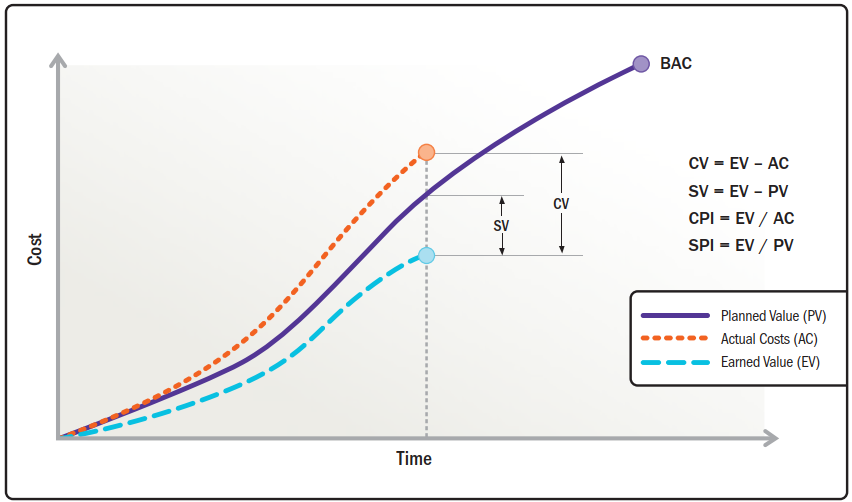
\includegraphics[width=0.9\textwidth]{svCvMetricsGraph.png}
    \attribution{PMBOK 7}
\end{center}

Тут проект отстаёт от исходного плана, при этом выходит за запланированный график финансовых расходов, то есть проект в беде. CV и SV отрицательны, CPI и SPI меньше 1, хотя внешне всё хорошо~--- за бюджет проекта мы не вышли и сроков не превысили.

\subsubsection{Прогноз показателей по методике Earned Value}

Смотря на график выше, можно понять, что проекту вряд ли станет сильно лучше в будущем, поскольку половину времени разработки проекта тренд на превышение бюджета и сроков сохранялся. Однако естественно желание количественно оценить, насколько всё плохо, чтобы принять меры (например, спасти проект, пересогласовав условия контракта или найдя дополнительные инвестиции). В этом помогут прогнозирующие метрики.

\begin{itemize}
    \item Прогноз для завершения (Estimate to complete, ETC)~--- ожидаемая стоимость окончания всех оставшихся работ. Самый простой способ её посчитать~--- вычесть из общего бюджета стоимость уже выполненных работ и поделить на Cost performance index (т.е. $ETC = (BAC - EV) / CPI$). Показывает, сколько денег нам ещё надо, чтобы закончить (разумеется, в предположении, что CPI мы мониторим в течение некоторого времени, достаточно точно его знаем и не предполагаем, что он сильно изменится в будущем~--- что для большинства проектов предположение слишком смелое, но прогнозы в целом неблагодарное дело).
    \item Прогноз по завершении (Estimate at completion, EAC)~--- ожидаемая стоимость всех работ в целом. Считается просто как $AC + ETC$, то есть сколько денег мы уже потратили и сколько ожидаем ещё потратить. В каком-то смысле это настоящий бюджет по окончании проекта, тогда как BAC~--- это бюджет, который мы изначально планировали. Светлая цель~--- $EAC <= BAC$.
    \item Отклонение при завершении (Variance at completion, VAC)~--- прогноз разницы между фактическим и запланированным бюджетом. То есть $VAC = EAC - BAC$.
    \item Индекс производительности до завершения (To-complete Performance Index, TCPI)~--- показывает требуемую эффективность трат для достижения цели проекта ($TCPI =  ETC / (BAC - AC)$). Это желаемый CPI, чтобы не вылететь за бюджет. Если TCPI сильно больше CPI, то беда.
\end{itemize}

Вот график, показывающий прогнозные метрики:

\begin{center}
    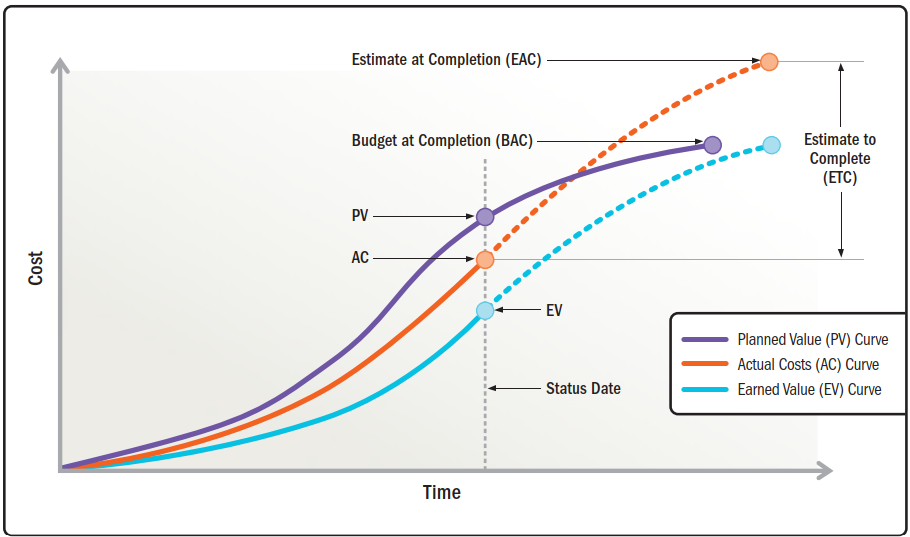
\includegraphics[width=0.9\textwidth]{eacEtcMetricsGraph.png}
    \attribution{PMBOK 7}
\end{center}

Тут судя по тому, что EV отстаёт от PV, проект выйдет за расчётное время, и по нашей оценке выйдет и за бюджет, несмотря на то, что сейчас потраченные средства меньше расчётных. Это видно по графику, AC обгоняет EV, так что CPI меньше 1, мы тратим деньги менее эффективно и так, поэтому вышли бы за бюджет даже если бы уложились по времени. Но перенос дедлайна на более поздний срок заставит нас ещё дольше оплачивать труд команды разработки, что сделает проект ещё менее финансово состоятельным.

Опять-таки, без количественных оценок и прогнозов график выглядит прекрасно~--- есть небольшое отставание по срокам, но ведь потом нагоним, да? Зато меньше денег потратили, чем планировали, сэкономили на разработке, увеличив чистую прибыль проекта, мы молодцы, да? Хорошая иллюстрация пользы подхода с Earned Value относительно \enquote{давайте мы на диаграмме Гантта отметим сделанные задачи и посмотрим, сколько из низ левее текущего дня, сколько правее}.

\subsubsection{Бизнес-метрики}

К сожалению, большинство проектов в IT делается не для того, чтобы принести пользу, а для того, чтобы заработать денег, поэтому одни из самых важных метрик~--- это бизнес-метрики, которые измеряют по сути только одно~--- сколько мы на этом заработали, не принимая во внимание такие детали, как оценку задач, процент выполнения и т.п. Поскольку в рыночной экономике стоимость чего угодно часто критически зависит от фейков в соцсетях, все подобного рода оценки весьма условны, но именно на них основываются решения людей, которые решают, быть или не быть проекту. Вот ключевые такие метрики:

\begin{itemize}
    \item Соотношение затрат и выгод~--- отношение ожидаемой ценности для бизнеса к стоимости проекта. Стоимость проекта мы можем оценить по методикам выше, а вот с ожидаемой ценностью всё сложнее. Если это внутренний инструмент компании, то мы можем посчитать, сколько времени он сэкономит сотрудникам, помножить на зарплату сотрудников, помножить на планируемый срок эксплуатации, и получить примерную оценку в деньгах (так что если вы год пишете практику, чтобы Юрию Литвинову сэкономить 15 минут в семестр на, скажем, загрузке текстов работ на сайт кафедры, то Cost-Benefit-показатель вашего проекта минимален). Если продукт планируется продавать, можно оценить объём рынка, оценить планируемый охват рынка, прикинуть цену, которую покупатели будут готовы отдать за продукт, и исходя из этого принимать решение о бюджете проекта и стартовать его вообще или нет. Если это заказная разработка, то Cost-Benefit-анализ уже проделал заказчик, иначе он бы к вам не пришёл.
    
    Обратите внимание, что показатель Cost-Benefit может быть меньше 1 (то есть проект заведомо убыточен), если есть другие веские причины его делать, кроме получения прибыли~--- например, вы можете быть обязаны его делать по требованиям регулятора (например, если вы не стаёте бухгалтерскую отчётность, вас закроют), или проект может иметь большое социальное значение (например, правительство часто субсидирует убыточные предприятия, чтобы люди не лишились работы и не пошли грабить зазевавшихся путников), или есть политические причины взяться за проект (например, установить доверительные отношения с заказчиком в надежде урвать заказ пожирнее).
    \item Запланированная ценность относительно актуальной ценности~--- какую ценность мы планировали предоставить заказчику против того, что получилось. Это может быть регулярно мониторящаяся метрика, если проект имеет внятный \enquote{Roadmap} и имеет частые релизы. Ценность сложно оценить, но понятно, что если мы обещали хорошо, а сделали так себе, это повлечёт существенный репутационный ущерб.
    \item Возврат инвестиций (Return of investment, ROI)~--- отношение текущей стоимости проекта к затратам. Например, вы вложились в проект на старте, потратив миллион рублей за долю в 10\% компании, проект \enquote{взлетел} и его купила другая компания (например, Microsoft) за сто миллионов рублей, при продаже вы вышли из компании, получив свои 10\%, то есть десять миллионов. Ваш ROI~--- 1000\%, что очень неплохо. Текущую стоимость проекта оценить сложно (и по факту стоимость определяется тем, за сколько его купили), а предсказать ещё сложнее, но если вам кажется, что ROI будет меньше 1, проект не стоит стартовать или в него вкладываться.
    \item Чистая приведённая стоимость (Net Present Value, NPV)~--- разница между инвестициями и прибылью от проекта. Не очень хороший показатель в плане того, что проект в ходе разработки, скорее всего, прибыли вообще не приносит, так что это применимо либо при прогнозировании, либо к уже эксплуатирующимся системам. Зато оценка NPV на некий интервал времени в будущем~--- хороший способ сказать, сколько именно денег вы заработаете (и, кстати, важный фактор при оценка стоимости проекта). Поскольку такого рода вещи считаются на значимых временных интервалах, надо делать поправку на инфляцию (поэтому и \enquote{приведённая} в названии метрики), и технически оно считается не так прямолинейно, как хотелось бы (точные правила расчёта легко найти в интернете, так что не будем тут про это).
\end{itemize}

\subsubsection{Метрики заинтересованных сторон}

Довольно важный показатель~--- это степень удовлетворённости пользователей. Однако поскольку удовлетворённость пользователей в деньги непосредственно не конвертируется, то считают обычно в каком-то смысле производную метрику~--- Net promoter score, NPS. Это балл от -100 до 100, показывающий, насколько пользователь готов рекомендовать продукт другим людям. Высокий NPS показывает высокую удовлетворённость, лояльность, и напрямую влияет на продажи продукта, если ваш проект продуктовый, поскольку пользователи работают в качестве бесплатной рекламы, приводя новых пользователей в геометрической прогрессии.

Однако важно также мониторить и удовлетворённость команды~--- проблемы с командой оказывают большее влияние на проект, чем любые технические сложности. Это можно делать с помощью диаграмм настроения, например, таких:

\begin{center}
    
\includegraphics[width=0.7\textwidth]{moodChart.png}
    \attribution{PMBOK 7}
\end{center}

Это весьма субъективный показатель, его можно несколько объективизировать и превратить в численную метрику с помощью регулярных (но не очень!) опросов, в духе \enquote{Оцените от 1 до 5 степень своего согласия со следующими утверждениями:}

\begin{itemize}
    \item \enquote{Я чувствую, что моя работа вносит свой вклад в достижение общих результатов}
    \item \enquote{Я чувствую, что меня ценят}
    \item \enquote{Я доволен тем, как моя проектная команда работает вместе}
\end{itemize}

Также важным показателем для больших проектов является текучка кадров~--- насколько часто люди от вас уходят. То, что люди уходят, совершенно нормально~--- они могут хотеть расти в другой области, кто-то предложил большую зарплату, может, люди просто переехали или что-то ещё. Но если люди уходят из проекта при первой возможности, это очень плохо, потому что на введение человека в проект тратятся значительные ресурсы. Кстати, текучку кадров очень легко считать, это не какая-то абстрактная мораль команды.

\subsection{Интерпретация метрик}

Метрики сами по себе бесполезны, на их основании должны приниматься решения. Для принятия решений можно визуализировать финансовые показатели на двумерном графике, где по горизонтальной оси откладывается Schedule variance, а по вертикальной~--- Cost variance: 

\begin{center}
    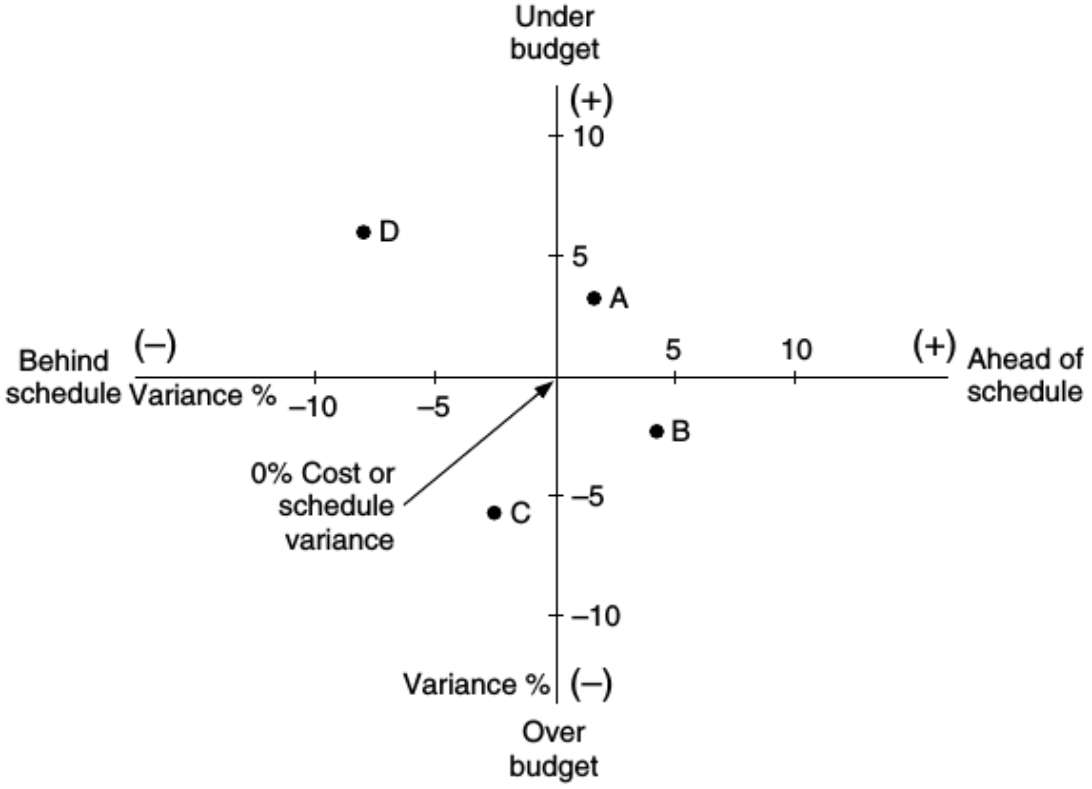
\includegraphics[width=0.8\textwidth]{varianceGraph.png}
\end{center}

Если проект попадает в правый верхний квадрант, всё хорошо, если в левый нижний, всё плохо. Однако само по себе это и так понятно, гораздо полезнее разметить этот график прямоугольниками, например, вот так:

\begin{center}
    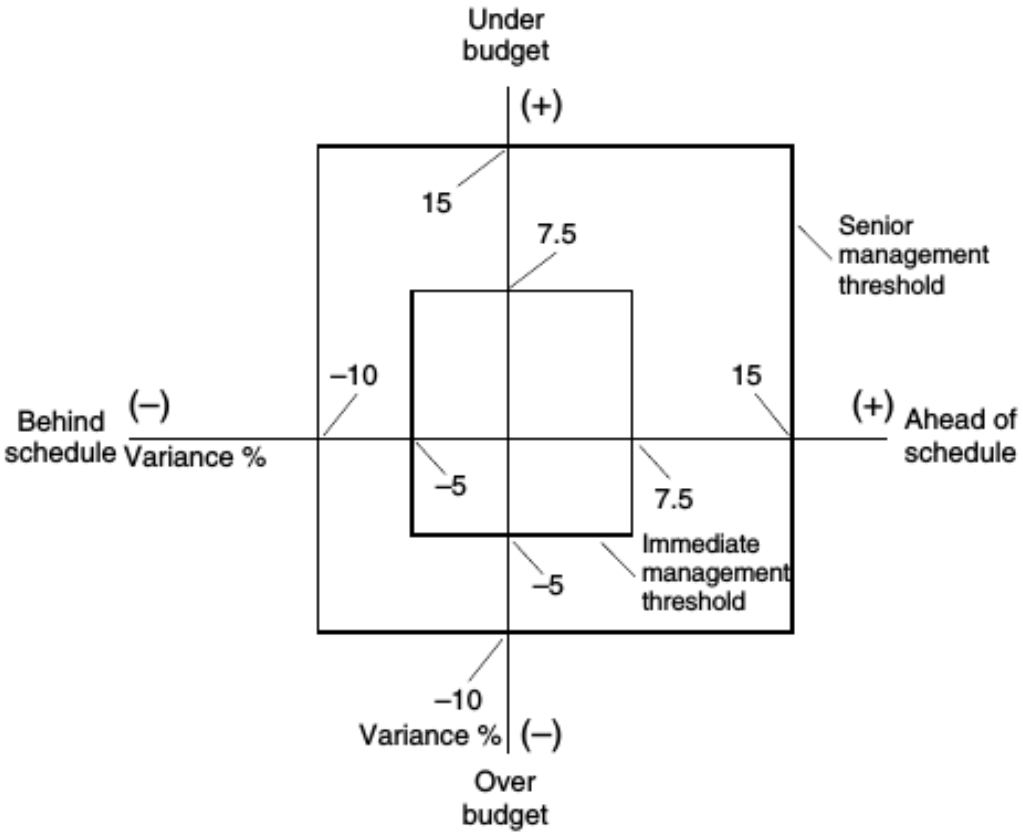
\includegraphics[width=0.7\textwidth]{escalationThresholds.png}
\end{center}

Эти прямоугольники называются порогами эскалации. Если проект выходит за границы внутреннего прямоугольника, мы как менеджер проекта начинаем принимать меры по компенсации доступными нам способами (про которые ниже). Если проект выходит за границы внешнего прямоугольника, мы эскалируем проблему до высшего руководства~--- это означает, что своими силами мы разрешить ситуацию не смогли и надо принимать решения, которые мы принимать не уполномочены.

Обратите внимание, что прямоугольники смещены относительно начала координат~--- это не удивительно, если всё хорошо, беспокоиться не о чем. Однако даже в правом верхнем квадранте тоже есть пороги эскалации~--- если проект существенно опережает график или существенно дешевле, чем ожидалось, это открывает некоторые возможности. Мы можем их использовать в рамках нашего проекта (например, расширить функциональные требования, надеясь увеличить охват аудитории), либо доложить вышестоящему начальству, чтобы оно могло использовать это в интересах всей компании.

\subsection{Трудности при применении метрик}

Есть известные проблемы, с которыми сталкиваются даже опытные руководители, полагающиеся на метрики при управлении проектом:

\begin{itemize}
    \item Эффект Хоторна (Hawthorne effect)~--- сам факт измерения меняет поведение измеряемой системы. Более того, измеряемая система, если в ней имеется обратная связь по результатам измерений, начинает подстраиваться под способ измерения. Поэтому выбор измеряемых метрик сам по себе является элементом управления, что можно использовать во благо~--- выбирать метрики, достижение которых действительно позитивно скажется на проекте. А можно выбрать метрики неудачно и люди будут, например, заниматься накруткой себе индекса Хирша\footnote{К теме лекции это не имеет отношения, но если что, индекс Хирша~--- это максимальное N для которого верно, что у данного учёного есть N статей, которые процитировали не менее N раз. По идее показывает продуктивность и состоятельность работы учёного, но если от него зависят зарплаты и кадровые решения, то... Ходят легенды о конференции, где 20 студентов в соавторстве со своим научником представили 20 работ, и через год на той же конференции другие 20 студентов представили 20 работ, каждая из которых ссылалась на каждую из 20 работ прошлого года.}, а не реальной научной работой. Можно разорвать цикл обратной связи, то есть метрики собирать, но нигде их не показывать и не принимать на их основании каких-то видимых для наблюдаемой системы решений, но тогда от таких метрик мало толку. Если метрики не показывать, но решения на их основании принимать, система всё равно научится их обманывать.
    \item Пустые метрики~--- метрики, на основании которых не принимаются никакие решения. Часто собираются из соображений показать, какой вы старательный менеджер и как любите строгий учёт. Но собирать метрики дорого, а собирать бесполезные метрики~--- непростительная роскошь.
    \item Деморализация из-за недостижимых целевых показателей. Если у метрики есть цель и этой цели команда никак не может достигнуть, команда впадёт в депрессию (иногда подсознательно, мораль будет снижаться, но даже сама команда не будет понимать, почему). Ставить светлые заведомо недостижимые цели можно, но нужно явно их таковыми декларировать и нужно ставить и достижимые цели, чтобы команда получала позитивную обратную связь.
    \item Неправильное использование метрик:
    \begin{itemize}
        \item фокус на неважных метриках, когда мы собираем много метрик, но по какой-то причине принимаем решения на основании второстепенных, игнорируя существенные для проекта;
        \item фокус на достижении кратковременных целевых показателях в ущерб долгосрочным;
        \item \enquote{достигательство}~--- когда команда или менеджер стараются увеличить легко достижимые, пусть и не вполне релевантные успеху проекта метрики, игнорируя суть вещей. Например, тот же индекс Хирша, если поставить себе цель его увеличить, можно относительно легко увеличить, но он никому не нужен сам по себе, его суть~--- измерять эффективность научной деятельности, и вот эту эффективность надо увеличивать на самом деле. Если вы будете премировать за количество коммитов, практически наверняка получите коммиты с заменой табуляций на пробелы и пробелов на табуляции.
    \end{itemize}
    \item Предвзятость подтверждения (Confirmation bias)~--- это свойство человеческого мышления, если мы сформировали у себя в голове некую модель мира, то мы будем выбирать из экспериментальных фактов (в нашем случае метрик) те, которые её подтверждают, и принижать значение тех, что её опровергают, списывая на случайность, временность, ошибки измерения и т.п. Причём делаем мы это неосознанно.
    \item Корреляция не влечёт причинность (Correlation does not imply causation)~--- если нарисовать на одном графике количество пиратов в Карибском море и среднегодовую температуру по земному шару, станет очевидно, что нужно срочно возрождать пиратство, чтобы остановить глобальное потепление. Нельзя делать выводы только по тому, что какие-то метрики коррелируют друг с другом~--- это может быть просто случайностью, или причины корреляции несколько более сложны, чем те, которые вы смогли найти и принять на их основе управленческие решения.
\end{itemize}

\section{Балансирование равновесия проекта}

\subsection{Треугольник равновесия}

В каждом проекте есть три основных момента:

\begin{itemize}
    \item стоимость;
    \item ресурсы (люди, компьютеры, время...);
    \item функциональность.
\end{itemize}

\begin{center}
    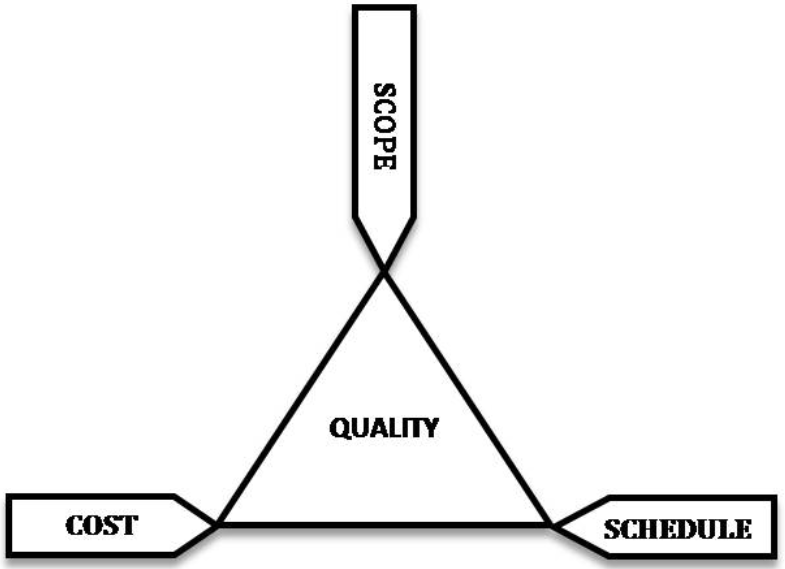
\includegraphics[width=0.4\textwidth]{balanceTriangle.png}
\end{center}

Если вы измените одну из этих переменных, то это неизбежно отразится и на оставшихся переменных тоже. Действительно, если вы увеличите функциональность вашего проекта (добавите новые фичи), то вы не сможете это сделать с той же стоимостью за то же самое время. Это очевидно, поскольку у вас работы больше стало. Если у вас становится меньше денег или людей, то это, разумеется, скажется на качестве продукта, вы не реализуете то же самое количество функциональности за то же самое время. Точно так же, чтобы обеспечить такое же качество продукта за более короткий период времени, придется увеличить стоимость. Задача менеджера проекта, состоит в том, чтобы сбалансировать эти переменные, чтобы создать оптимальное равновесие между ценой и качеством.

Есть еще одна интересная картинка~--- то же самое, но для заказчика:

\begin{center}
    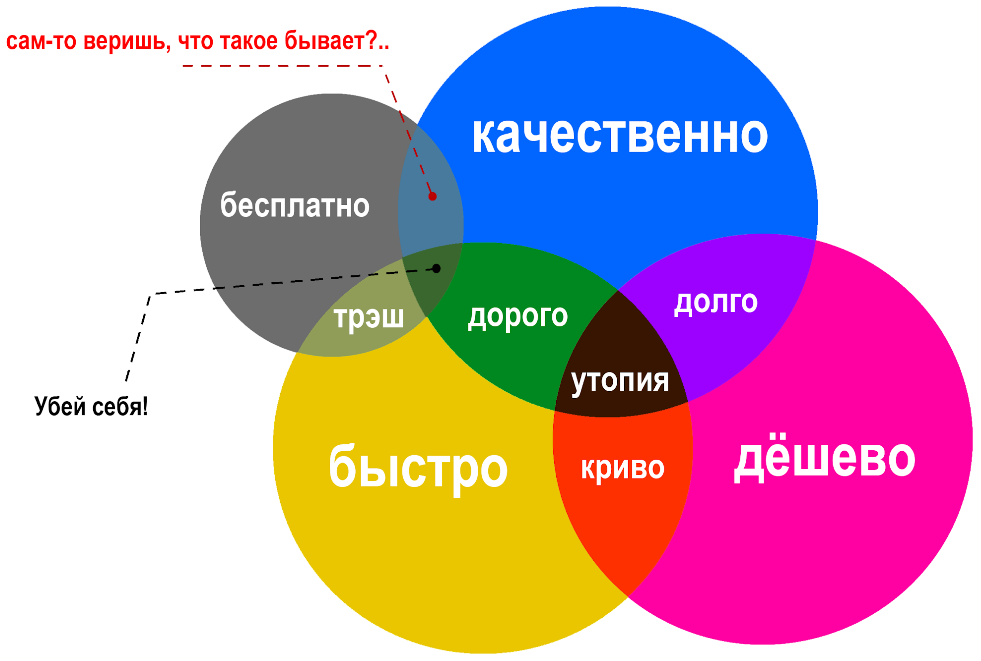
\includegraphics[width=0.6\textwidth]{balanceTriangleExplained.png}
\end{center}

Не бывает быстро, качественно и дешево. Если вы делаете быстро и дешево~--- получается криво; дешево и качественно~--- долго; быстро и качественно~--- дорого и т.д.

Равновесие в проекте нужно сохранять постоянно (до завершения работы над проектом). Эта работа делается на разных уровнях: проекта, бизнес-целей, компании.

\paragraph{Балансирование на уровне проекта.} Изменения, которые никак не повлияют на сроки, бюджет, количество людей и т.д., менеджер может принимать сам, они не требуют авторизаций или разрешений. Пока это остается в рамках ограничений, с проектом можно делать всё, что угодно.

\paragraph{Балансирование на уровне бизнес-целей.} Изменения на уровне проекта возможны не всегда, иногда их просто недостаточно, и требуется сдвигать одну или несколько вершин треугольника равновесия. В таком случае нужно принимать решения на уровне бизнес-целей, а это требует согласования с заказчиком и/или руководством компании.

\paragraph{Балансирование на уровне компании.} Изменения на уровне компании~--- глобальные изменения. Подобные изменения принимаются уже руководством компании, которое должно балансировать сразу все проекты компании. Например, у одного проекта может быть резко урезан бюджет с целью выделения дополнительных средств другому, более критичному проекту. Данный уровень в лекции мы затрагивать не будем.

\subsection{Балансирование на уровне проекта}

\paragraph{Повторная переоценка задач.} Первое, что стоит попробовать сделать при балансировке на уровне проекта~--- повторно оценить задачи. То есть, уже в процессе работы ещё раз пересмотреть график проекта и задачи в нем. Возможно сейчас у вас больше информации, чем на этапе изначальной оценки, и оценки получатся точнее. Вполне возможно, какие-то задачи были переоценены, а некоторые вообще уже потеряли актуальность.

Однако при переоценке задач следует действовать очень осторожно: нельзя выдавать желаемое за действительное. Например, если хочется сократить бюджет, то возникает большой соблазн обмануться и избавиться от задач, которые на самом деле важны.

Плюсы: потенциальное сокращение сроков, бюджета, объема работ. Но если новой информации или требований у вас не появилось, то этот метод вряд сильно сработает. Тем не менее, к нему стоит время от времени возвращаться.

\paragraph{Перераспределение задач критического пути.} При балансировании проекта всегда стоит уделять особое внимание задачам на критическом пути в сетевом графике.

Можно попробовать увеличить число людей, занятых работой над критическими задачами, задавшись целью сделать их быстрее. Обычно привлекают людей, работающих над другими задачами. Однако, такой подход может скрывать массу подводных камней. Во-первых, добавление людей к задаче не всегда повышает продуктивность работы, например, если задачи были распланированы с оптимальным количеством людей. Кроме того, следует иметь в виду, насколько хорошо задачи параллелятся. Если хорошо, то добавление новых людей к решению этой задачи, скорее всего, принесет пользу. Но чаще всего задачи нельзя распараллелить. Например: задача разработки архитектуры, запланированная на одного архитектора, не будет сделана существенно быстрее архитектором и четырьмя программистами. Добавление людей к таким задачам в худшем случае только замедлит работу, а в лучшем~--- принесёт незначительное улучшение.

Следует также иметь в виду, что при привлечении новых людей к решению задачи продуктивность каждого из работников может упасть. Соответственно, расходы проекта растут. Ну и при переводе человека из одного проекта в другой может потребоваться время на его обучение и адаптацию.

Таким образом, при перераспределении людей по задачам нужно учитывать следующие моменты.

\begin{itemize}
    \item Квалификация работников: не стоит заставлять дизайнера писать тесты или проектировать архитектуру.
    \item Действительно ли это поможет сократить время работы? Не будет ли человек лишним? 
    \item Как поменялись резервы в задачах? Не изменился ли критический путь?
\end{itemize}

\paragraph{Добавление людей в проект.} При добавлении людей в проект задачи практически никогда не начинают резко делаться быстрее, чем до этого, т.к. при добавлении человека в уже запущенный проект его нужно хотя бы как-то обучить и адаптировать, контролировать его работу. Это приводит к трате времени других людей в проекте, соответственно, сбивается график проекта: человек, который мог бы в это время делать задачи проекта, тратит своё время на нового сотрудника (а сам новый сотрудник ещё не работает). В графике продуктивности команды при добавлении новых людей почти всегда происходит сначала небольшой спад.

Исходя из этого, в краткосрочной перспективе добавление новых людей в проект невыгодно (только если добавляется не какой-нибудь супер-специалист, который хорошо знает команду, предметную область и проект). Почти всегда добавление новых людей~--- это инвестиция в будущее проекта.

Резервы для добавления обычно ищутся внутри компании, но обычно из резерва можно найти не самых опытных людей. Поэтому не стоит надеяться на то, что в критической ситуации можно резко добавить ещё крутых специалистов, и всё пойдёт быстрее.

Привлечение новых людей хорошо работает в проектах с открытым исходным кодом, поскольку в подобных проектах, как правило, обычно строго древовидная иерархия и с новым человеком работает локальная часть этой иерархии. Однако, например, в agile проектах это может работать хуже, поскольку новый человек будет обращаться за помощью ко всем (т.к. может) и тем самым затормозит прогресс проекта. О том, как подобный подход может разрушить планы даже очень крупных компаний, можно почитать, например, тут: \url{https://www.eurogamer.net/stormlands-and-the-million-man-raid-obsidians-cancelled-xbox-one-exclusive} (дата обращения: 27.03.2023).

\paragraph{Привлечение экспертов в проект.} Эксперты бывают внутренние (изнутри компании) и внешние.

Внутренний эксперт~--- специалист внутри компании, временно снятый со своего основного проекта. Такой эксперт привлекается, как правило, чтобы помочь с какой-то локальной проблемой, а потом вернуться к своей основной работе. Плюсы: человек лоялен к проекту/компании, обладает требуемыми компетенциями и готов их вам предоставить в лучшем виде. Например, эксперт настраивает базу данных, делает это быстро и грамотно, время внутри команды не тратится. Но, во-первых, эксперт~--- человек, он тоже может совершить ошибку при настройке, может не уложиться в сроки и т.д. Во-вторых, никаких компетенций в области конкретной задачи, для решения которой привлекли эксперта, командой проекта не приобретается, т.к. всё сделал сторонний человек.

Что же делать, если снова случится такая проблема? Если бы было потрачено время на обучение своего сотрудника, то при необходимости этот сотрудник мог бы снова решить проблему. Таким образом, в долгосрочной перспективе лучше обучать своих специалистов.

С целью избежания подобных ситуаций (а также с целью повышения компетенций команды) при привлечении эксперта со стороны, его нужно заставить передавать знания. Вряд ли это будет встречено с охотой, но неким образом эксперт всё же должен быть вовлечён в процесс планирования. Можно заставить эксперта участвовать в статус-митингах, попросить провести семинар и т.д. В таком случае привлечение эксперта работает хорошо, и при возникновении проблемы, схожей с той, для решения которой был привлечён эксперт, команда проекта уже будет иметь хотя бы некоторые знания, связанные с решением возникшей задачи.

Внешний эксперт~--- то же самое, но с компетенциями всё обстоит ещё хуже, поскольку это полностью сторонний человек, которого можно попросту не найти, если вдруг проблема возникла снова (или же при решении были допущены ошибки).

Предпочтительный вариант~--- растить собственных экспертов. Это осуществляется либо с привлечением внутренних экспертов компании, либо же приглашением людей со стороны, которые будут обучать членов команды. Следует специализировать людей внутри команды в конкретных областях. Со временем они вполне сами могут стать экспертами (если не уйдут от вас в другой проект).

\paragraph{Аутсорсинг частей проекта.} Аутсорсинг~--- передача части проекта на разработку сторонней компании. При подобном подходе возникают две проблемы: помимо неприобретённой экспертизы, вы получаете зависимость от сторонней компании. Можно даже не догадываться, что происходит в той компании, которой отдана часть проекта, и у менеджера проекта существенно меньше возможностей контролировать процесс разработки. Аутсорсинг~--- довольно экстремальная вещь: или всё идёт хорошо, или всё идет плохо, а команда об этом и не подозревает. Нужно стараться контролировать процесс выполнения работы над частью проекта, отданной \enquote{на растерзание} другой компании. Из очевидных плюсов, аутсорсинг позволяет избежать проблем с квалификациями своих разработчиков. Например, когда нужно сделать приложения под все платформы, а программистов под iOS в команде нет, и заводить их не хочется. В таком случае аутсорсинг~--- очень выгодное решение.

\paragraph{Сверхурочная работа.} Ещё один часто приходящий на ум вариант повышения продуктивности~--- заставить членов команды работать больше. Казалось бы, всё выглядит очень оптимистично: пусть есть $X$ часов в неделю суммарно при работе программистов по $40$ часов. Если заставить их работать по $60$ часов в неделю, получим $1.5 * X$. Кроме того, не нужно добавлять новых людей, обучать их и т.д., просто члены команды будут работать дольше. Да и дополнительное время они будут работать в нерабочее время, когда офис не так сильно заполнен людьми, так что будут меньше отвлекаться и т.п.

Однако, на самом деле всё вовсе не так хорошо. Конечно, это нормально, если перед дедлайном приходится, например, поработать в выходные, чтобы сделать релиз в понедельник, но если переработки происходят регулярно, то программисты начинают \enquote{выгорать}. Люди начинают уставать, продуктивность падает. Но мы про это уже говорили в одной из прошлых лекций.

При решении интеллектуальных задач производительность очень сильно страдает от усталости. Заставить человека, занимающегося интеллектуальным трудом, работать больше, чем обычно~--- почти всегда путь к плохим последствиям. Как писал ДеМарко, на каждый час переработки приходится примерно час недоработки. И это он ещё оптимист. Не бывает так, чтобы люди волшебным образом стали работать в 1.5-2 раза больше. Фанатизм в работе сказывается на здоровье, усталости. Заканчивается это часто возросшей апатией человека и нежеланием делать вообще что-либо. Таким образом очень легко теряются программисты. В долгосрочной перспективе переработки крайне невыгодны.

Грамотный менеджер должен не заставлять команду программистов работать \enquote{на часик подольше}, а как раз наоборот, следить за тем, чтобы не было систематических переработок. Сознательные переработки~--- признак непрофессионализма. Если человек каждый день засиживается на работе, то, скорее всего, у него проблемы с тайм-менеджментом. Скорее всего, в течение дня он тратит свое время на что-то никак не связанное с работой. Здесь, опять же, бывают исключения, но таких людей (\enquote{фанатиков}) очень мало, и с ними, как правило, всё понятно. И они тоже выгорают.

\paragraph{Снижение качества проекта.} \emph{Качество проекта никогда не следует понижать.} Конечно, соблазн велик, но последствия всегда весьма плачевны. Например, можно сэкономить на тестах, но взамен поймать кучу рандомных багов. Даже в краткосрочной перспективе не стоит понижать качество продукта, т.к., скорее всего, будет сделан очень некачественный продукт, который потом придется переделывать, на что уйдет больше времени, особенно если это придётся делать через несколько месяцев после завершения работы. Возможно даже, что придется переписывать весь проект заново. Гораздо дешевле не допускать ошибок, чем их исправлять. Жертвовать можно чем угодно, но не качеством. Даже если вы сдадите проект, потерянную репутацию потом будет крайне сложно восстановить.

\subsection{Балансирование проекта на уровне бизнес-целей}

\paragraph{Пересмотр границ проекта.} Когда приходит понимание, что в заданные сроки и бюджет требуемую функциональность реализовать не получается, стоит посмотреть, а нельзя ли как-то подвинуть границы проекта, нельзя ли от какой-то функциональности более-менее безболезненно избавиться (хотя бы на данном этапе). Подобные решения требуют обоснованных переговоров с заказчиком и часто основываются на анализе требований и сценариев использования продукта. Поэтому их можно осуществлять только на уровне бизнес-целей компании. Ну и не всегда можно безболезненно выбросить какую-то функциональность: всё же продукты должны обладать какими-то особенностями, чтобы иметь на рынке конкурентное преимущество. А такие особенности чаще всего и являются тем, что сложно в реализации (иначе у конкурентов оно уже было бы тоже реализовано).

\paragraph{Подстраивание проекта под дедлайны.} Часто бывает так, что у продуктов есть фиксированный дедлайн, в который команда не укладывается, однако дедлайн имеет первостепенную важность. В таком случае следует разбить период времени до дедлайна на несколько этапов, по завершении каждого из которых будет согласовываться дальнейшее направление развития проекта. В каждой ключевой точке фиксируется функциональность на ближайший этап, при достижении следующей планируется следующий этап и т.д. В итоге набор функциональности можно определять динамически.

Подобный подход работает далеко не всегда. Например, заказчик может захотеть добавить что-то, что просто не вписывается в текущую архитектуру. Также заказчик может хотеть работать по более традиционной схеме и отказаться брать на себя ответственность за разбиение проекта на этапы и определение функциональности на них.

\paragraph{Работа на опережение.} Для работ, которые нельзя сделать параллельно, можно применить следующий подход. Допустим, у нас есть задача A, а также задача B, которая должна быть сделана по завершении работы над задачей A. В таком случае можно начать делать B ещё до завершения A. Например, можно начать реализовывать отдельные компоненты проекта до того, как архитектура будет закончена целиком.

При таком подходе надо действовать аккуратно, т.к. есть большая вероятность того, что придется переделывать решение. Это связано с тем, что принимаются предположения касательно реализации в духе \enquote{скорее всего, это будет так}, однако гарантии этого нет и в результате всё может быть совсем иначе.

Если всё сложится удачно, данный подход может позволить получить хорошую выгоду, но возможен и негативный исход, который приведет к уходу в минус. Тем не менее, при грамотном анализе рисков подобная \enquote{хитрость} может помочь. С помощью такой техники можно сэкономить до 30-40\% времени.

\paragraph{Incremental delivery.} Поэтапная разработка: поставлять заказчику изменения в продукте небольшими партиями. Такой подход работает далеко не со всеми проектами (и уж тем более не со всеми заказчиками). Например, это точно не сработает с большими, монолитными системами. Но, как правило, такое бывает довольно редко, а вот заказчики, которые не хотят так работать, встречаются весьма часто.

\paragraph{Прототипирование.} Прототипирование~--- мощный инструмент, суть которого заключается в том, что до начала работы над проектом создается черновой вариант проекта целиком (или каких-то его частей), но без особого внимания к качеству и деталям. Такой прототип создается просто для теста и получения опыта/знаний о предметной области, поэтому, когда работа над ним завершена, нужно избавиться от него и сделать заново, но уже хорошо.

Этот подход вынуждает потратить больше денег на разработку (приходится делать многое дважды), но, с другой стороны, позволяет снять риски и потратить меньше денег на исправление ошибок. Следует отметить, что очень важно избавиться от первоначального прототипа по завершению его разработки, а не использовать его в качестве основания для \enquote{настоящего} проекта, поскольку прототип, как уже было сказано выше, делается на скорую руку и, скорее всего, будет целиком и полностью основан на \enquote{костылях}.

\paragraph{Снижение прибыльности проекта.} Пожертвовать прибыльностью проекта~--- последний шаг, к которому стоит прибегнуть, если ничего больше не работает. Это подразумевает уход проекта \enquote{в минус}, заём денег у других проектов, и т.д. Другой вариант~--- жертвовать репутацией и выпускать продукт ненадлежащего качества, позже дедлайна, и т.д. Далеко не все компании согласны на такое, поэтому чаще прибегают к потери прибыли проекта, но сохранению репутации.

\end{document}
